% HOPES & EXPECTATIONS
As a potential improvement over the employed \(\text{MC}^3\text{KS}\) sampler we will devise a new hybrid MCMC sampling scheme.
Since the scheme will be based on data augmentation (DA), henceforth it will be referred to as \(\text{MC}^3\text{DA}\).
% CLASSICALLY -> HEREIN
Traditionally DA can be a powerful tool for enhancing the computational efficiency of MCMC posterior sampling \cite{MCMC:Tanner1987,MCMC:Dyk2001,MCMC:Dyk2003}.
Instead we will herein utilize DA as a means to reformulate the multilevel model calibration problem in such a complementary way,
that it allows for more adequate likelihood estimations in view of \cref{eq:JAIS:PerfectData:MSE}.
In turn this promises an enhancement of the posterior fidelity through \cref{eq:JAIS:MCMC:MHCorrection}.
% NORMAL REFERENCE RULE
The approach will also allow for automatic kernel bandwidth selection based on a classical yet well-approved criterion, namely the normal reference rule \cite{Statistics:Silverman1986}.
This is appealing since it avoids the cumbersome procedure of tuning free algorithmic parameters of the KDE that was described in \cref{sec:JAIS:Analysis:LikelihoodEstimation}.
\par % PARTIAL DATA AUGMENTATION
Rather than directly sampling the posterior of the QoI \((p_2,\bm{\theta}_1,\bm{\theta}_{45})\), one can sample the posterior of an augmented number of unknowns
\((\tuple{p_{1,i}},p_2,\bm{\theta}_1,\bm{\theta}_{45})\) and obtain the posterior of the QoI by subsequently marginalizing over nuisance \(\tuple{p_{1,i}}\).
% EFFICIENCY
Presuming that sampling from \(\pi(\tuple{p_{1,i}},p_2,\bm{\theta}_1,\bm{\theta}_{45} \cond \tuple{\perfect{y}_i},\bm{\theta}_3)\) is ``easier'' to accomplish
than straightforwardly sampling from \(\pi(p_2,\bm{\theta}_1,\bm{\theta}_{45} \cond \tuple{\perfect{y}_i},\bm{\theta}_3)\), a de facto improvement is achieved.
% TERMINOLOGY: PARTIAL DATA AUGMENTATION
The introduction of \(\tuple{p_{1,i}}\) as auxiliary variables is a partial form of data augmentation.
% MOTIVATION: NUMERICAL EFFICIENCY -> POSTERIOR FIDELITY
As indicated by preliminary problem analyses, the forward model \(h_1\) seems to be in such a strong way dependent on its input \(p_1\),
that the data \(\tuple{\perfect{y}_i}\) can be inverted for the unknown \(\tuple{p_{1,i}}\), under uncertainty of the remaining unknowns.
% ADDITIONAL INSIGHT
Even though \(\tuple{p_{1,i}}\) are not QoI this provides additional insight into to inverse problem posed.
% LIKELIHOOD ESTIMATION
Moreover the likelihood function corresponding to partial data augmentation can be estimated more adequately.
% HIGHER FIDELITY
Presumably, within a feasible computation time, the aforementioned facts will allow to sample \(\pi(\tuple{p_{1,i}},p_2,\bm{\theta}_1,\bm{\theta}_{45} \cond \tuple{\perfect{y}_i},\bm{\theta}_3)\)
with higher fidelity than sampling \(\pi(p_2,\bm{\theta}_1,\bm{\theta}_{45} \cond \tuple{\perfect{y}_i},\bm{\theta}_3)\).
% FORMALISM
We will introduce the formalism of partial data augmentation below.

\subsection{Augmented multilevel model}
If the unknowns \((p_2,\bm{\theta}_1,\bm{\theta}_{45})\) of the Bayesian multilevel model \cref{eq:JAIS:PerfectData:Model} are augmented by experiment-specific realizations \(\tuple{p_{1,i}}\),
then the collective of unknowns \((\tuple{p_{1,i}},p_2,\bm{\theta}_1,\bm{\theta}_{45})\) has to be explicitly taken into account.
% PRIOR DISTRIBUTION
The associated Bayesian prior is given as
\begin{equation} \label{eq:JAIS:Augmentation:Prior}
  \pi \big( \tuple{p_{1,i}},p_2,\bm{\theta}_1,\bm{\theta}_{45} \big)
  = \left( \prod\limits_{i=1}^n f_1(p_{1,i} \cond \bm{\theta}_1) \right)
  \pi_2(p_2) \, \pi_1(\bm{\theta}_1) \, \pi_{45}(\bm{\theta}_{45}).
\end{equation}
This distribution comprises both parametric and structural prior knowledge.
Given an appropriate probability model \(f(\perfect{y}_i \cond p_{1,i},p_2,\bm{\theta}_{45},\bm{\theta}_3)\) of random variables
\((\perfect{Y}_i \cond p_{1,i},p_2,\bm{\theta}_{45},\bm{\theta}_3)\),
the corresponding \textit{augmented likelihood} follows as
% LIKELIHOOD FUNCTION
\begin{equation} \label{eq:JAIS:Augmentation:Likelihood}
  \mathcal{L} \big( \tuple{\perfect{y}_i} \cond \tuple{p_{1,i}},p_2,\bm{\theta}_{45},\bm{\theta}_3 \big)
  = \prod\limits_{i=1}^n f (\perfect{y}_i \cond p_{1,i},p_2,\bm{\theta}_{45}, \bm{\theta}_3).
\end{equation}
% TRANSFORMED DENSITY
The definition of the augmented likelihood \cref{eq:JAIS:Augmentation:Likelihood} rests upon a probability model
\((\perfect{Y}_i \cond p_{1,i},p_2,\bm{\theta}_{45},\bm{\theta}_3) \sim f(\perfect{y}_i \cond p_{1,i},p_2,\bm{\theta}_{45},\bm{\theta}_3)\).
Analogous to the propagated uncertainty in \cref{eq:JAIS:PerfectData:PushForwardDensity}, such a model is established through a transformed random variable \(\mathcal{M}_{p_{1,i},p_2} (P_3,P_4,P_5)\) with a density function
\begin{equation} \label{eq:JAIS:Augmentation:PushForwardDensity}
  f (\perfect{y}_i \cond p_{1,i},p_2,\bm{\theta}_{45},\bm{\theta}_3)
  = \int\limits_{0}^{1} \int\limits_{-\infty}^{+\infty} \int\limits_{-\infty}^{+\infty} \delta \big( \perfect{y}_i - \mathcal{M}_{p_{1,i},p_2} (p_3,p_4,p_5) \big)
  \, f_3(p_{3} \cond \bm{\theta}_3) \, f_{45} \big( (p_{4},p_{5}) \cond \bm{\theta}_{45} \big)
  \, \mathrm{d} p_3 \, \mathrm{d} p_4 \, \mathrm{d} p_5.
\end{equation}
Here \(\delta\) denotes the Dirac delta function and \(\mathcal{M}_{p_{1,i},p_2} \colon (p_3,p_4,p_5) \mapsto \mathcal{M}(p_{1,i},p_2,p_3,p_4,p_5)\)
formalizes the map that the forward model \(\mathcal{M} \equiv h_1\) defines for fixed inputs \((p_{1,i},p_2)\) and functional arguments \((p_3,p_4,p_5)\).
% POSTERIOR
With the combined parametric and structural prior \cref{eq:JAIS:Augmentation:Prior} and the augmented likelihood \cref{eq:JAIS:Augmentation:Likelihood},
the augmented posterior of the unknowns \((\tuple{p_{1,i}},p_2,\bm{\theta}_1,\bm{\theta}_{45})\) is according to Bayes' law proportional to
\begin{equation} \label{eq:JAIS:Augmentation:Posterior}
  \pi \big( \tuple{p_{1,i}},p_2,\bm{\theta}_1,\bm{\theta}_{45} \cond \tuple{\perfect{y}_i},\bm{\theta}_3 \big)
  \propto \mathcal{L} \big( \tuple{\perfect{y}_i} \cond \tuple{p_{1,i}},p_2,\bm{\theta}_{45},\bm{\theta}_3 \big)
  \, \pi \big( \tuple{p_{1,i}},p_2,\bm{\theta}_1,\bm{\theta}_{45} \big).
\end{equation}
% MARGINAL POSTERIOR
Since we are not interested in inferring experiment-specific realizations \(\tuple{p_{1,i}}\) per se, they are treated as nuisance.
Similar to the marginalization \cref{eq:JAIS:Multilevel:MarginalPosterior} the posterior of the QoI \((p_2,\bm{\theta}_{1},\bm{\theta}_{45})\)
is thus found by integrating the posterior \cref{eq:JAIS:Augmentation:Posterior} as follows
\begin{equation} \label{eq:JAIS:Augmentation:MarginalPosterior}
  \pi \big( p_2,\bm{\theta}_1,\bm{\theta}_{45} \cond \tuple{\perfect{y}_i},\bm{\theta}_3 \big)
  = \int\limits_{0}^{1} \ldots \int\limits_{0}^{1} \pi \big( \tuple{p_{1,i}},p_2,\bm{\theta}_1,\bm{\theta}_{45} \cond \tuple{\perfect{y}_i},\bm{\theta}_3 \big)
  \, \mathrm{d} \tuple{p_{1,i}},
\end{equation}
where \(\mathrm{d} \tuple{p_{1,i}} = \mathrm{d} p_{1,1} \ldots \mathrm{d} p_{1,n}\) as before.
% MATHEMATICAL EQUIVALANCE
Both of the distributions \cref{eq:JAIS:PerfectData:Posterior,eq:JAIS:Augmentation:MarginalPosterior} equivalently define the desired posterior
\(\pi(\bm{m},\bm{\theta}_{\bm{X}} \cond \tuple{\perfect{\bm{y}}_i},\bm{\theta}_{\bm{Z}}) \equiv \pi(p_2,\bm{\theta}_1,\bm{\theta}_{45} \cond \tuple{\perfect{y}_i},\bm{\theta}_3)\).
While \cref{eq:JAIS:PerfectData:Posterior} straightforwardly conditions via
\(\pi(p_2,\bm{\theta}_1,\bm{\theta}_{45} \cond \tuple{\perfect{y}_i},\bm{\theta}_3) \propto \mathcal{L}(\tuple{\perfect{y}_i} \cond p_2,\bm{\theta}_1,\bm{\theta}_{45},\bm{\theta}_3) \, \pi(p_2,\bm{\theta}_1,\bm{\theta}_{45})\),
\cref{eq:JAIS:Augmentation:Posterior,eq:JAIS:Augmentation:MarginalPosterior} provide a rearrangement where nuisance variables \(\tuple{p_{1,i}}\) are firstly factored out before they are eventually eliminated.
\par % PRACTICAL COMPUTATION
Even though this scheme of data augmentation leads to a higher-dimensional estimation problem, it may be computationally advantageous.
In practice the marginal \cref{eq:JAIS:Augmentation:MarginalPosterior} can be computed by sampling the joint distribution \cref{eq:JAIS:Augmentation:Posterior} and simply discarding samples of \(\tuple{p_{1,i}}\),
i.e.\ the multi-dimensional integral does not have to be calculated explicitly.
% RELATION BETWEEN AUGMENTATION AND ``PERFECT'' DATA
Writing the compound distribution
\begin{equation} \label{eq:JAIS:Augmentation:DensityRelation}
  f (\perfect{y}_i \cond p_2,\bm{\theta}_1,\bm{\theta}_{45},\bm{\theta}_3) = \int\limits_{0}^{1} f (\perfect{y}_i \cond p_{1,i},p_2,\bm{\theta}_{45},\bm{\theta}_3) \, f (p_{1,i} \cond \bm{\theta}_1) \, \mathrm{d} p_{1,i}
\end{equation}
establishes the connection between the transformed likelihood \(\mathcal{L}(\tuple{\perfect{y}_i} \cond p_2,\bm{\theta}_1,\bm{\theta}_{45},\bm{\theta}_3)\) of the form \cref{eq:JAIS:PerfectData:Likelihood}
and the augmented likelihood \(\mathcal{L}(\tuple{\perfect{y}_i} \cond \tuple{p_{1,i}},p_2,\bm{\theta}_{45},\bm{\theta}_3)\) in \cref{eq:JAIS:Augmentation:Likelihood}.
The relation \cref{eq:JAIS:Augmentation:DensityRelation} suggests that \(f (\perfect{y}_i \cond p_{1,i},p_2,\bm{\theta}_{45},\bm{\theta}_3)\) could be a ``simplified'' version of
the ``complex'' distribution \(f (\perfect{y}_i \cond p_2,\bm{\theta}_1,\bm{\theta}_{45},\bm{\theta}_3)\) that was exemplarily shown in \cref{pre:JAIS:TransformedLikelihood}.
Ideally it would be a unimodal distribution that resembles a Gaussian.
Indeed in this case the augmented likelihood could be estimated more adequately than the transformed one.
Consequently, the QoI-marginal of the induced limiting distribution of the \(\text{MC}^3\text{DA}\) scheme can be expected to be closer to the true posterior
than the long-run distribution of the \(\text{MC}^3\text{KS}\) approach.
\par % DIRAC DELTA
An augmented model can be analogously defined when latent variables other than \(\tuple{p_{1,i}}\) are introduced as auxiliary variables.
The more variables are introduced, the smaller the variance of the target density similar to \cref{eq:JAIS:Augmentation:PushForwardDensity} is expected to be.
In the case that all variables \((\tuple{p_{1,i}},\tuple{p_{3,i}},\tuple{p_{4,i}},\tuple{p_{5,i}})\) are jointly introduced, the conditional distribution of the data would even shrink to a Dirac delta
\(f (\tilde{y}_i \cond p_{1,i},p_2,p_{3,i},p_{4,i},p_{5,i}) = \delta(\perfect{y}_i-\mathcal{M}_{p_{1,i},p_2,p_{3,i},p_{4,i},p_{5,i}})\).
Note that for if ``imperfect'' data \(y_i = \perfect{y}_i + \varepsilon_i\) would be involved, a proper distribution would still be defined as
\(f (y_i \cond p_{1,i},p_2,p_{3,i},p_{4,i},p_{5,i}) = f_{E_i} (y_i -\mathcal{M}_{p_{1,i},p_2,p_{3,i},p_{4,i},p_{5,i}})\).
In fact this exactly defines the distribution \cref{eq:JAIS:Multilevel:Model:Data} of the a joint problem in \cref{eq:JAIS:Multilevel:Model}.
% MOTIVATION FOR \(p_1\)
The motivation for augmenting with \(\tuple{p_{1,i}}\) is the expectation that this provides a convenient trade-off between fidelity and feasibility,
i.e.\ likelihood evaluations are optimally facilitated with respect to the implied increase in dimensionality.

\subsection{Augmented likelihood estimation}
% LIKELIHOOD ESTIMATION
In practical terms the augmented likelihood \cref{eq:JAIS:Augmentation:Likelihood} can be estimated analogously to \cref{eq:JAIS:PerfectData:KernelSmoothedLikelihood}.
To that end the response density \(f (\perfect{y}_i \cond p_{1,i},p_2,\bm{\theta}_{45},\bm{\theta}_3)\) is estimated for each \(p_{1,i}\) and evaluated for the given responses \(\perfect{y}_i\).
Hence a KDE-based estimate of the augmented likelihood as a function of \((\tuple{p_{1,i}},p_2,\bm{\theta}_{45})\) is given as
\begin{gather} \label{eq:JAIS:Augmentation:KernelSmoothedLikelihood}
  \begin{aligned}
  \hat{\mathcal{L}}_{\mathrm{DA}} \big( \tuple{\perfect{y}_i} \cond \tuple{p_{1,i}},p_2,\bm{\theta}_{45},\bm{\theta}_3 \big)
  = \prod\limits_{i=1}^n \left( \frac{1}{K} \sum\limits_{k=1}^{K} \mathcal{K}_{h_i} \left( \perfect{y}_i-\perfect{y}_i^{(k)} \right) \right), \\
  \text{with} \;\, \left\{
  \begin{aligned}
    p_{3,i}^{(k)} &\sim f_3 (p_{3,i}^{(k)} \cond \bm{\theta}_3), \\
    \big( p_{4,i}^{(k)},p_{5,i}^{(k)} \big) &\sim f_{45} \big( (p_{4,i}^{(k)},p_{5,i}^{(k)}) \cond \bm{\theta}_{45} \big), \\
    \perfect{y}_i^{(k)} &= \mathcal{M}_{p_{1,i},p_2}(p_{3,i}^{(k)},p_{4,i}^{(k)},p_{5,i}^{(k)}), \\
    h_i &= (\nicefrac{4}{3K})^{1/5} \, \hat{\sigma}_i.
  \end{aligned}
  \right.
  \end{aligned}
\end{gather}
For \(k=1,\ldots,K\) inputs \(p_{3,i}^{(k)} \sim f_3 (p_{3,i}^{(k)} \cond \bm{\theta}_3)\) and \((p_{4,i}^{(k)},p_{5,i}^{(k)}) \sim f_{45}((p_{4,i}^{(k)},p_{5,i}^{(k)}) \cond \bm{\theta}_{45})\)
are sampled from the corresponding population distributions, responses \(\perfect{y}_i^{(k)} = \mathcal{M}_{p_{1,i},p_2}(p_{3,i}^{(k)},p_{4,i}^{(k)},p_{5,i}^{(k)})\) are computed accordingly.
Furthermore \(\hat{\sigma}_i\) denotes the standard deviation of the response samples \((\perfect{y}_i^{(1)},\ldots,\perfect{y}_i^{(K)})\).
% I-SPECIFIC ESTIMATION
Note that in \cref{eq:JAIS:Augmentation:KernelSmoothedLikelihood} the density \(f(\perfect{y}_i \cond p_{1,i},p_2,\bm{\theta}_{45}, \bm{\theta}_3)\) is individually estimated for each \(p_{1,i}\) with \(i=1,\ldots,n\).
% ALGORITHMIC TUNING
The number of samples for each of these estimations is set to \(K=10^3\) and selection of the bandwidths follows the normal reference rule \(h_i = (\nicefrac{4}{3K})^{1/5} \, \hat{\sigma}_i\).
\par % RV-COMPARISON
Let us compare the transformed densities \cref{eq:JAIS:PerfectData:PushForwardDensity,eq:JAIS:Augmentation:PushForwardDensity}.
The random variable \(\mathcal{M}_{p_2} (P_1,P_3,P_4,P_5) \sim f(\perfect{y}_i \cond p_2,\bm{\theta}_1,\bm{\theta}_{45},\bm{\theta}_3)\)
is conditioned on \(\bm{\theta}_1\) and involves the uncertainty of \(P_1 \sim f_1(p_{1} \cond \bm{\theta}_1)\).
In contrast \(\mathcal{M}_{p_{1,i},p_2} (P_3, \allowbreak P_4,P_5) \sim f(\perfect{y}_i \cond p_{1,i},p_2,\bm{\theta}_{45},\bm{\theta}_3)\)
is conditioned on the realization \(p_{1,i}\) and does not bear reference to \(\bm{\theta}_1\).
% SIMPLER DENSITY
Hence \(f(\perfect{y}_i \cond p_2,\bm{\theta}_1,\bm{\theta}_{45},\bm{\theta}_3)\) is the broader and more complex density,
whereas \(f(\perfect{y}_i \cond p_{1,i},p_2,\bm{\theta}_{45},\bm{\theta}_3)\) is simpler and easier to estimate.
% BIAS & VARIANCE % POSTERIOR FIDELITY
In turn, likelihood estimations for \(\text{MC}^3\text{DA}\) are less biased and have a smaller variance than for \(\text{MC}^3\text{KS}\).
Thus the approach promises a higher degree of posterior fidelity.
% VISUALIZATION
In \cref{pre:JAIS:AugmentedLikelihood} the density \(f(\perfect{y}_i \cond p_{1,i},p_2,\bm{\theta}_{45},\bm{\theta}_3)\) is shown for values
\((p_2,\bm{\theta}_{45})_{\mathrm{high}}\) and \((p_2,\bm{\theta}_{45})_{\mathrm{low}}\) that have been chosen as the same values already used in \cref{pre:JAIS:TransformedLikelihood}.
Following our final results, the value \(p_{1,i}\) has been exemplarily chosen as the posterior mean of \(p_{1,i}\) with \(i=36\).
% COMPARISON: TRANSFORMED vs AUGEMENTED
When comparing \cref{pre:JAIS:TransformedLikelihood,pre:JAIS:AugmentedLikelihood} one can clearly see the essential difference between the densities
\(f(\perfect{y}_i \cond p_2,\bm{\theta}_1,\bm{\theta}_{45},\bm{\theta}_3)\) and \(f(\perfect{y}_i \cond p_{1,i},p_2,\bm{\theta}_{45},\bm{\theta}_3)\).
The latter is distinctly simpler and clearly better resembling a Gaussian density.
% COMPARISON: HIGH vs LOW POSTERIOR
Moreover the densities for (hyper)parameter values of high and low posterior evidence only negligibly overlap.
% DATA CONSISTENCY
It can also be seen that the chosen values \(p_{1,36}\) and \((p_2,\bm{\theta}_{45})_{\mathrm{high}}\) lead to a response density which is consistent with the observation \(\perfect{y}_{36}\).
% MC^3KS: EVALUATION OF THE AUGMENTED LIKELIHOOD
\begin{figure}[htbp]
  \centering
  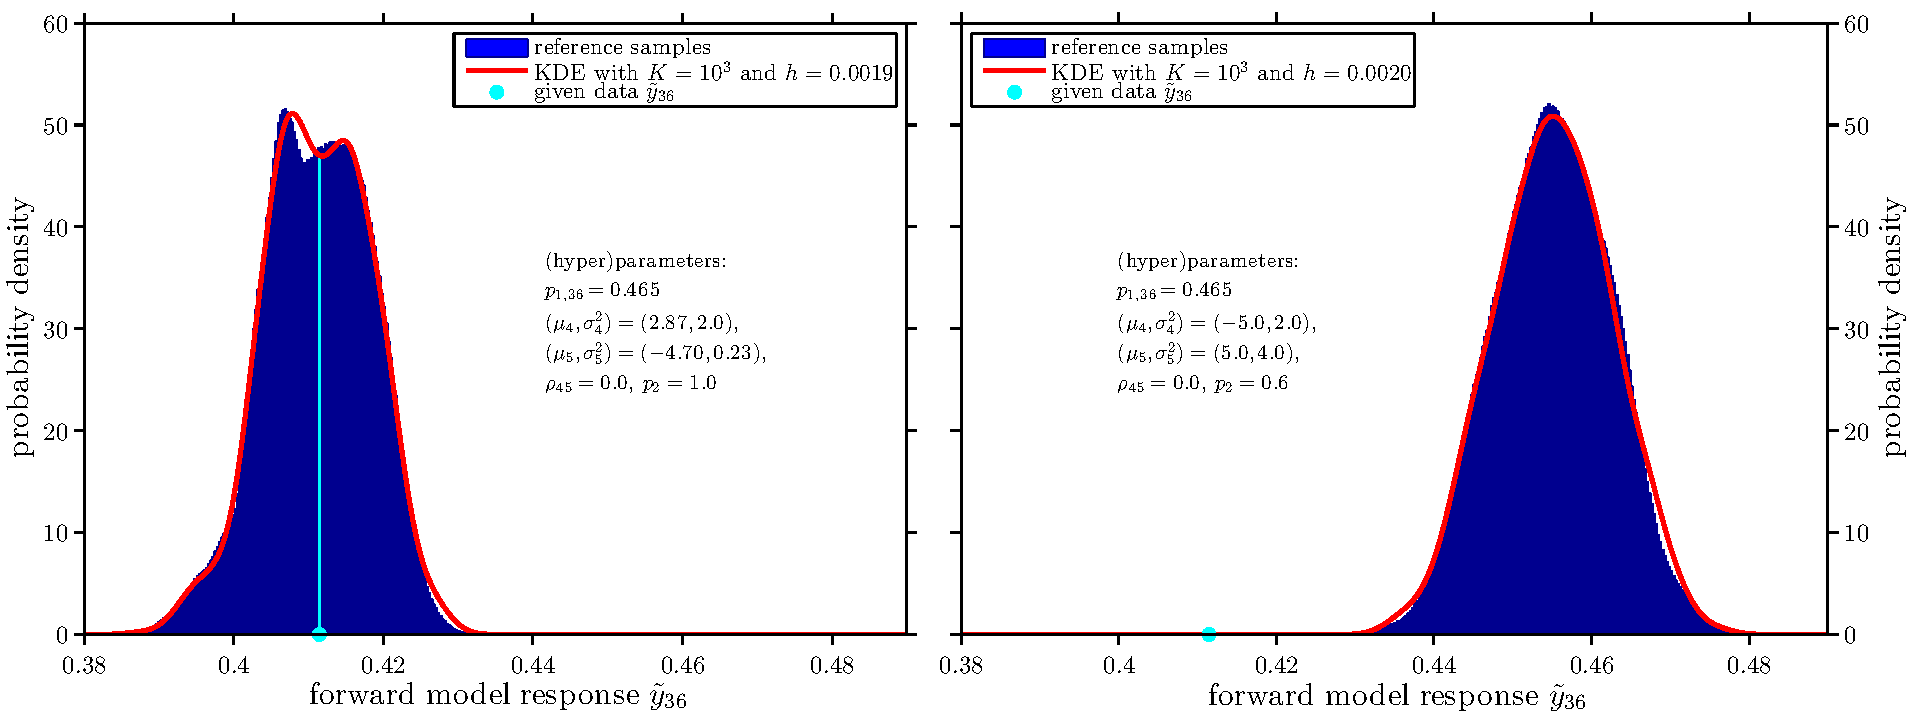
\includegraphics[width=\JAISfigWidth]{fig_JAIS_DA_AugmentedLikelihood}
  \caption[Estimation of \(f(\perfect{y}_{36} \cond p_{1,36},p_2,\bm{\theta}_{45},\bm{\theta}_3)\)]{Estimation of \(f(\perfect{y}_{36} \cond p_{1,36},p_2,\bm{\theta}_{45},\bm{\theta}_3)\).
           Evaluating the augmented likelihood \cref{eq:JAIS:Augmentation:Likelihood} for \(\text{MC}^3\text{DA}\) is based on the response density \cref{eq:JAIS:Augmentation:PushForwardDensity}.
           For \(p_{1,36} = 0.465\) and two different values of the (hyper)parameters \((p_2,\bm{\theta}_{45})_{\mathrm{high}}\) and \((p_2,\bm{\theta}_{45})_{\mathrm{low}}\)
           a KDE of \(f(\perfect{y}_{36} \cond p_{1,36},p_2,\bm{\theta}_{45},\bm{\theta}_3)\) with \(K=10^3\) is shown.
           The bandwidths \(h=0.0019\) and \(h=0.0020\) were automatically selected according to the normal reference rule.
           Histograms with a larger number \(K=10^7\) are shown for reference purposes.
          }
  \label{pre:JAIS:AugmentedLikelihood}
\end{figure}

\subsection{MCMC}
% DATA AUGMENTATION
The augmented posterior \cref{eq:JAIS:Augmentation:Posterior} is explored by means of a suitable \(\text{MC}^3\text{DA}\) sampler.
% BLOCKWISE
Updating is done in blocks \(\tuple{p_{1,i}}\), \((\mu_1,\sigma^2_1)\), \((p_2)\), \((\mu_4)\), \((\mu_5)\) and \((\sigma^2_4,\sigma^2_5,\rho_{45})\).
Each \(p_{1,i}\) in the block \(\tuple{p_{1,i}}\) is concurrently updated with a random walk Metropolis sampler based on independent Gaussian proposals with standard deviation \(\sigma_{p_{1,i}} = 0.01\).
As before the remaining blocks are initialized in the middle of the corresponding epistemic intervals and updated with independent prior proposals.
% ACCEPTANCE RATES
Acceptance rates amounted to ca.\ \(\unit[10]{\%}\) for \(\tuple{p_{1,i}}\), \((p_2)\), and \((\mu_5)\),
\(\unit[15]{\%}\) for \((\mu_4)\) and \((\sigma^2_4,\sigma^2_5,\rho_{45})\), and \(\unit[30]{\%}\) for \((\mu_1,\sigma^2_1)\).
% BETA REQUIREMENT
A number of \(10219\) proposals in the last-mentioned block were rejected due to violating \(\alpha_1,\beta_1>1\).
% CONVERGENCE
We start with preliminary MCMC runs with \(K=10^3\) and constant bandwidths \(h_i=0.02\) in order to identify the posterior modes of \(\tuple{p_{1,i}}\).
Experiment-specific realizations \(\tuple{p_{1,i}}\) are initialized in the middle of their epistemic intervals and converge within ca.\ \(1000\) MCMC iterations.
The initial convergence and final posterior of an experiment-specific realization \(p_{1,i}\) with \(i=10\) are shown in \cref{pre:JAIS:p1Convergence}.
This shows that individual experiment-specific realizations \(\tuple{p_{1,i}}\) can indeed be inferred.
% DRAWBACK
The danger of the approach is that missing further posterior modes of \(\tuple{p_{1,i}}\) would alter the sampled posteriors of the remaining unknowns, above all the one of \(\bm{\theta}_1\).
% CONVERGENCE CHECKS
Convergence checks have therefore been accomplished by initializing \(\tuple{p_{1,i}}\) within admissible regions of the parameter space that have not been visited in previous runs.
Ultimately the chains converged to the same posterior modes which were found before.
% ADDED REMARK
We conclude that the parameter space has been properly explored.
% MC^3DA: IDENTIFIABILITY & CONVERGENCE OF \(p_{1,i}\)
\begin{figure}[htbp]
  \centering
  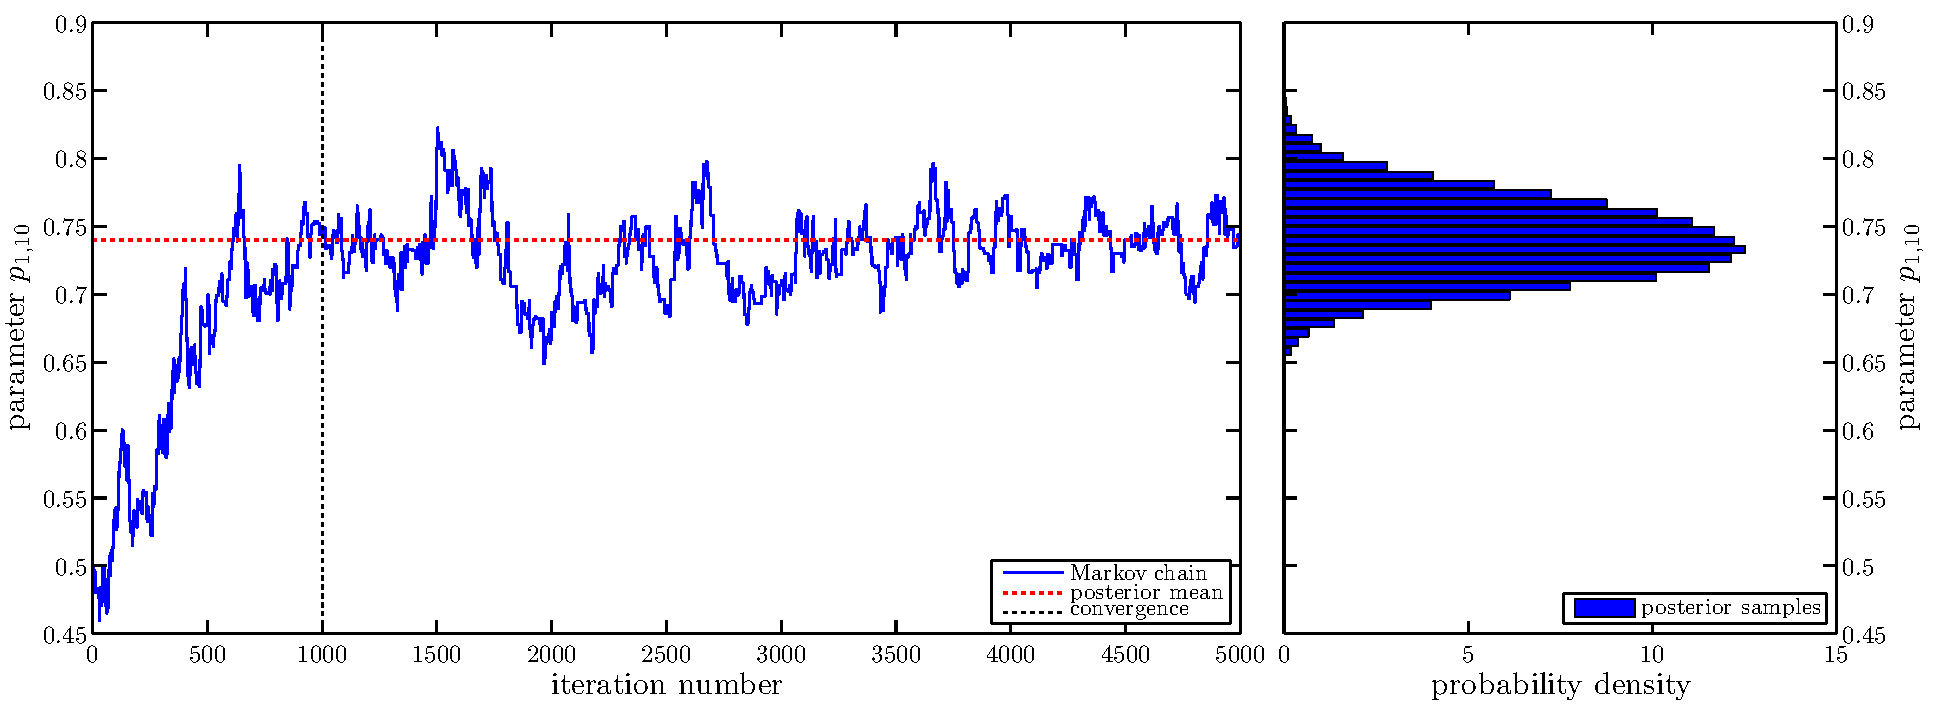
\includegraphics[width=\JAISfigWidth]{fig_JAIS_DA_p1Convergence}
  \caption[Convergence and identifiability of \(p_{1,10}\)]{Convergence and identifiability of \(p_{1,10}\).
           With \(N=10^5\) iterations of the \(\text{MC}^3\text{DA}\) algorithm the augmented posterior \cref{eq:JAIS:Augmentation:Posterior} is explored by analyzing \(\tuple{\perfect{y}_i}_{1 \leq i \leq 50}\).
           For a preliminary run with \(K=10^3\) and fixed \(h_i=0.02\), i.e.\ without automatic bandwidth selection, a trace plot of the converging Markov chain of an experiment-specific \(p_{1,10}\) is shown.
           After convergence within ca.\ \(1000\) iterations the Markov chain samples the corresponding posterior around its mean.
          }
  \label{pre:JAIS:p1Convergence}
\end{figure}
\par % ADDITIONAL INSIGHT
We point out that although partial data augmentation has been motivated by considerations of posterior fidelity, it also gives additional insight into the inverse problems posed.
Incidentally the posterior of experiment-specific realizations \(\tuple{p_{1,i}}\) is explored and its modes are identified.
Thus we have gained knowledge about unknown problem quantities that are not primary QoI.
% FINAL RUNS
Eventually we initialize the final sampler within the detected posterior modes of \(\tuple{p_{1,i}}\).
With \(K=10^3\) and automatic selection of the bandwidths \(h_i\) we draw \(N=10^5\) posterior samples.
Total execution time amounts to \(t \approx \unit[90]{h}\) on a single core.
% CONCLUSION
The resulting posterior marginals of the QoI are added to \cref{res:JAIS:Hyper1,res:JAIS:Param2Rho45,res:JAIS:Hyper4,res:JAIS:Hyper5}.
As compared to the results obtained by \(\text{MC}^3\text{KS}\) the posteriors found by \(\text{MC}^3\text{DA}\) have been slightly shrunk and evolved in structure.
Resting upon the assumption that the posterior modes of \(\tuple{p_{1,i}}\) have been correctly identified, we take this as an indication of a gain in posterior fidelity.
% POSTERIOR CORRELATION
In \cref{res:JAIS:2D:Mean1Sigma1Param1} two-dimensional posteriors are shown for \((\mu_1,\sigma^2_1)\) and \((\mu_1,p_{1,i})\) with \(i=19\).
The corresponding linear coefficients of correlation are found to be \(r_{\mu_1,\sigma^2_1} = -0.25\) and \(r_{\mu_1,p_{1,19}} = 0.19\).
Generally we find small linear correlations \(r_{\mu_1,p_{1,i}} \gtrsim 0\) between the mean hyperparameter \(\mu_1\) and experiment-specific realizations \(p_{1,i}\) for nearly all \(i=1,\ldots,n\).
% INTERPRETATION
This is plausible since higher values of \(\mu_1\) increase the plausibility of higher values of each \(p_{1,i}\) and vice versa.
% 2D POSTERIORS
\begin{figure}[htbp]
  \centering
  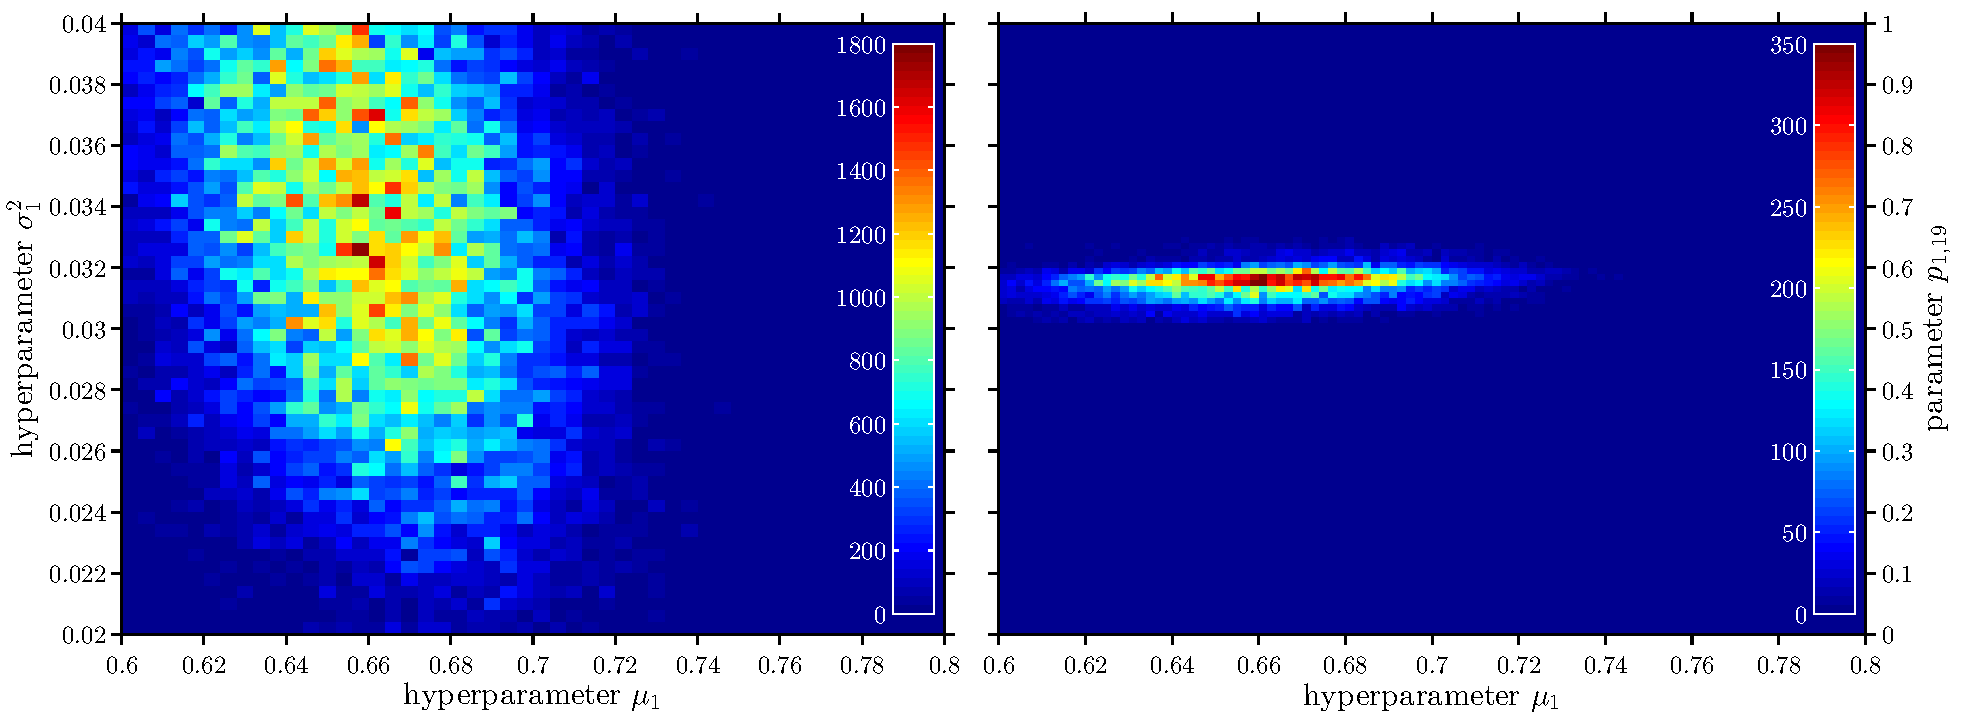
\includegraphics[width=\JAISfigWidth]{fig_JAIS_DA_2D_Mean1Sigma1Param1}
  \caption[2D posteriors of \((\mu_1,\sigma^2_1)\) and \((\mu_1,p_{1,19})\)]{2D posteriors of \((\mu_1,\sigma^2_1)\) and \((\mu_1,p_{1,19})\).
           Posterior projections that follow analyzing \(\tuple{\perfect{y}_i}_{1 \leq i \leq 50}\) are shown for \((\mu_1,\sigma^2_1)\) and \((\mu_1,p_{1,19})\).
           While the former can be compared to the corresponding posterior marginal in \cref{res:JAIS:2D:Mean1Sigma1Mean4} for \(\text{MC}^3\text{KS}\), the latter is appertain to \(\text{MC}^3\text{DA}\).
           Linear coefficients of correlation are found to be \(r_{\mu_1,\sigma^2_1} = -0.25\) and \(r_{\mu_1,p_{1,19}} = 0.19\).
          }
  \label{res:JAIS:2D:Mean1Sigma1Param1}
\end{figure}